% !TEX program = pdflatex
\documentclass[12pt,a4paper]{article}

% Packages
\usepackage[utf8]{inputenc}
\usepackage[margin=1in]{geometry}
\usepackage{graphicx}
\usepackage{xcolor}
\usepackage{titlesec}
\usepackage{fancyhdr}
\usepackage{tocloft}
\usepackage{hyperref}
\usepackage{listings}
\usepackage{enumitem}
\usepackage{tikz}
\usetikzlibrary{shapes.geometric,arrows.meta,positioning}
\usepackage{tcolorbox}
\usepackage{booktabs}
\usepackage{caption}
\usepackage{amssymb}

% Fix header height
\setlength{\headheight}{25pt}

% Color definitions
\definecolor{primarycolor}{RGB}{0,102,204}
\definecolor{secondarycolor}{RGB}{51,51,51}
\definecolor{accentcolor}{RGB}{0,153,204}
\definecolor{codebg}{RGB}{245,245,245}

% Hyperref setup
\hypersetup{
    colorlinks=true,
    linkcolor=primarycolor,
    filecolor=primarycolor,
    urlcolor=accentcolor,
    citecolor=primarycolor,
    pdftitle={Wireless Sensor Network for Robotic Fleet Coordination},
    pdfauthor={Team Members},
}

% Header and Footer
\pagestyle{fancy}
\fancyhf{}
\fancyhead[L]{\textcolor{primarycolor}{\small Wireless Sensor Network for Robotic Fleet Coordination}}
\fancyhead[R]{\textcolor{secondarycolor}{\small GIU - Winter 2025}}
\fancyfoot[C]{\textcolor{secondarycolor}{\thepage}}
\renewcommand{\headrulewidth}{0.5pt}
\renewcommand{\footrulewidth}{0.5pt}
\renewcommand{\headrule}{\hbox to\headwidth{\color{primarycolor}\leaders\hrule height \headrulewidth\hfill}}
\renewcommand{\footrule}{\hbox to\headwidth{\color{primarycolor}\leaders\hrule height \footrulewidth\hfill}}

% Section formatting
\titleformat{\section}
{\color{primarycolor}\normalfont\Large\bfseries}
{\color{primarycolor}\thesection}{1em}{}
[\titlerule]

\titleformat{\subsection}
{\color{accentcolor}\normalfont\large\bfseries}
{\color{accentcolor}\thesubsection}{1em}{}

\titleformat{\subsubsection}
{\color{secondarycolor}\normalfont\normalsize\bfseries}
{\color{secondarycolor}\thesubsubsection}{1em}{}

% Code listing style
\lstdefinestyle{cppstyle}{
    language=C++,
    backgroundcolor=\color{codebg},
    basicstyle=\ttfamily\footnotesize,
    keywordstyle=\color{primarycolor}\bfseries,
    commentstyle=\color{gray}\itshape,
    stringstyle=\color{accentcolor},
    numbers=left,
    numberstyle=\tiny\color{gray},
    stepnumber=1,
    numbersep=8pt,
    frame=single,
    rulecolor=\color{primarycolor},
    breaklines=true,
    breakatwhitespace=false,
    tabsize=2,
    showstringspaces=false,
    captionpos=b
}

\lstset{style=cppstyle}

% Custom tcolorbox styles
\tcbuselibrary{skins,breakable}
\newtcolorbox{infobox}{
    colback=primarycolor!5,
    colframe=primarycolor,
    fonttitle=\bfseries,
    title=Information,
    breakable,
    enhanced,
    attach boxed title to top left={yshift=-2mm,xshift=5mm},
    boxed title style={colback=primarycolor}
}

\newtcolorbox{notebox}{
    colback=accentcolor!5,
    colframe=accentcolor,
    fonttitle=\bfseries,
    title=Note,
    breakable,
    enhanced,
    attach boxed title to top left={yshift=-2mm,xshift=5mm},
    boxed title style={colback=accentcolor}
}

\newtcolorbox{codebox}[1]{
    colback=codebg,
    colframe=secondarycolor,
    fonttitle=\bfseries,
    title=#1,
    breakable,
    enhanced
}

% Document start
\begin{document}

% Remove header/footer from cover page
\thispagestyle{empty}

% ===================================
% COVER PAGE
% ===================================
\begin{titlepage}
    \centering
    
    \vspace*{1cm}
    
    \vspace{1cm}
    
    {\Large \textbf{German International University}\par}
    {\large Faculty of Engineering\par}
    {\large Major of Automation and Control\par}
    
    \vspace{1.5cm}
    
    {\color{primarycolor}\rule{\linewidth}{0.5mm}}\par
    
    \vspace{0.5cm}
    
    {\Huge \textbf{\textcolor{primarycolor}{Wireless Sensor Network}}\par}
    {\Huge \textbf{\textcolor{primarycolor}{for Robotic Fleet}}\par}
    {\Huge \textbf{\textcolor{primarycolor}{Coordination}}\par}
    
    \vspace{0.5cm}
    
    {\color{primarycolor}\rule{\linewidth}{0.5mm}}\par
    
    \vspace{1cm}
    
    {\Large Introduction to Computer Networks\par}
    {\Large Project Report\par}
    
    \vspace{2cm}
    
    \begin{minipage}{0.8\textwidth}
        \begin{center}
            {\large \textbf{Team Members}\par}
            \vspace{0.5cm}
            \begin{tabular}{ll}
                Hassan Yousef & 13006567 \\
                Pierre George Boshra & 13007351 \\
                Mohamed Walid & 13006513 \\
                Abdelhamid ElSharnouby & 13006294 \\
                Khaled Khaled & 14001048 \\
                Mahmoud Nasser & 13006342 \\
            \end{tabular}
        \end{center}
    \end{minipage}
    
    \vspace{1.5cm}
    
    {\large \textbf{Supervised by}\par}
    {\large Dr. Yasmine Zaghloul\par}
    {\large TA: Eng. Omar Hemeda\par}
    
    \vfill
    
    {\large Winter Semester 2025\par}
    {\large December 2025\par}
    
\end{titlepage}

% ===================================
% TABLE OF CONTENTS
% ===================================
\newpage
\tableofcontents
\thispagestyle{empty}

\newpage
\setcounter{page}{1}

% ===================================
% WEEK 1: RESEARCH & SETUP
% ===================================
\newpage
\section{Week 1: Research \& Setup}
\textit{November 17-23, 2025}

\subsection{Research Phase}

To establish a solid foundation for our project, we conducted comprehensive research utilizing multiple academic and expert resources. Our research methodology included:

\begin{itemize}[leftmargin=*]
    \item \textbf{Academic Database Search:} We performed extensive literature review using the Egyptian Knowledge Bank (EKB) database, searching for relevant research papers and technical documentation on wireless sensor networks, ESP-NOW protocol, mesh networking architectures, and robotic coordination systems.
    
    \item \textbf{Expert Consultation:} We consulted with Professor Yasmine Zaghloul, our course instructor, to discuss the project scope, technical feasibility, and recommended implementation approaches. Her guidance helped us refine our project objectives and identify potential challenges.
    
    \item \textbf{Technical Advisory:} We met with TA Omar Hemeda to discuss the practical aspects of the project implementation, including hardware selection, programming methodologies, and project timeline management.
    
    \item \textbf{Laboratory Support:} We worked closely with Lab Engineer Amr Khaled to understand the available laboratory resources, safety protocols, and equipment handling procedures necessary for our project development.
\end{itemize}

\subsection{ESP-NOW Protocol Learning}

To gain practical understanding of the ESP-NOW protocol, we studied the tutorial video "\textit{ESPNOW for beginners! \#ESP32 \#ESP8266}" available at:

\begin{center}
    \url{https://www.youtube.com/watch?v=Ydi0M3Xd_vs}
\end{center}

This resource provided valuable insights into:
\begin{itemize}[leftmargin=*]
    \item The fundamentals of ESP-NOW as a fast, connectionless peer-to-peer communication protocol
    \item Setting up ESP-NOW connections between multiple ESP32 devices
    \item Broadcasting and receiving data packets using callback functions
    \item MAC address handling and peer registration
\end{itemize}

\subsection{Hardware Setup}

We successfully configured the development environment for the ESP32 microcontrollers using the Arduino IDE. The setup process included:

\begin{itemize}[leftmargin=*]
    \item Installing the Arduino IDE (version 2.x)
    \item Adding ESP32 board support through the Boards Manager
    \item Installing necessary libraries: \texttt{esp\_now}, \texttt{WiFi}, \texttt{MPU6050\_6Axis\_MotionApps20}, \texttt{WebServer}, \texttt{SPIFFS}
    \item Testing basic functionality with simple sketch uploads
    \item Verifying serial communication for debugging purposes
\end{itemize}

\subsection{Project Architecture Plan}

After thorough analysis and team discussions, we finalized our system architecture as follows:

\begin{infobox}
\textbf{Hardware Configuration:}
\begin{itemize}[leftmargin=*]
    \item \textbf{3 ESP32 Microcontrollers:} Serve as the core processing and communication units
    \item \textbf{2 Remote-Controlled Toy Vehicles:} Provide the mobile platform for our robotic agents
    \item \textbf{Mesh Network Architecture:} All three ESP32 units communicate peer-to-peer via ESP-NOW, with one base station connected to PC for visualization
\end{itemize}
\end{infobox}

\begin{notebox}
\textbf{Sensor Configuration per Vehicle:}
\begin{itemize}[leftmargin=*]
    \item \textbf{HC-SR04 Ultrasonic Sensor:} Detects obstacles within 15cm range in the robot's forward direction
    \item \textbf{IR Sensor:} Detects whether the robot is on a white or black square for position tracking
    \item \textbf{MPU6050 IMU (Gyroscope + Accelerometer):} Determines robot orientation (Forward, Right, Backward, Left) using DMP processing
\end{itemize}
\end{notebox}

\subsection{System Design Specifications}

\subsubsection{Initial Robot Positions}
The robots start at predefined positions on the 4x4 grid:
\begin{itemize}[leftmargin=*]
    \item \textbf{Robot 1:} Position (4, 1) --- bottom-left corner
    \item \textbf{Robot 2:} Position (4, 4) --- bottom-right corner
\end{itemize}

\subsubsection{Network Topology}
The system implements a mesh-like network topology where all three ESP32 devices maintain peer-to-peer connections:
\begin{itemize}[leftmargin=*]
    \item Robot 1 $\leftrightarrow$ Robot 2 (direct communication)
    \item Robot 1 $\leftrightarrow$ Base Station
    \item Robot 2 $\leftrightarrow$ Base Station
    \item Re-broadcast mechanism ensures all nodes receive updates
\end{itemize}

\subsubsection{Mapping Area Design}
The operational environment consists of a 4x4 grid-based area:
\begin{itemize}[leftmargin=*]
    \item Alternating white and black squares (checkerboard pattern)
    \item IR sensor detects color transitions to track movement between cells
    \item Obstacles can be placed statically within the grid
    \item Each cell is identified by row (1-4) and column (1-4) coordinates
\end{itemize}

\subsubsection{Communication Flow}
\begin{enumerate}[leftmargin=*]
    \item When Robot 1 detects an obstacle, it sends coordinates to Robot 2
    \item Robot 2 updates its internal map and re-broadcasts to Robot 1 and Base Station
    \item When Robot 2 detects an obstacle, it sends coordinates to Robot 1
    \item Robot 1 updates its internal map and re-broadcasts to Robot 2 and Base Station
    \item Base Station aggregates all updates and displays the map on PC via web interface
\end{enumerate}

\subsection{AI Tools Integration}

The strategic utilization of AI-powered development tools played a crucial role in accelerating our project timeline and enhancing code quality:

\begin{infobox}
\textbf{ChatGPT Integration:}
\begin{itemize}[leftmargin=*]
    \item \textbf{Code Generation:} Assisted in generating boilerplate code for ESP-NOW initialization, sensor drivers, and data structure definitions
    \item \textbf{Debugging Support:} Provided insights for troubleshooting ESP32-specific issues and memory management
    \item \textbf{Documentation:} Helped structure technical documentation and explain complex networking concepts
    \item \textbf{Algorithm Optimization:} Suggested efficient approaches for map synchronization and re-broadcast logic
\end{itemize}
\end{infobox}

\begin{infobox}
\textbf{GitHub Copilot Integration:}
\begin{itemize}[leftmargin=*]
    \item \textbf{Real-time Code Completion:} Accelerated development with intelligent auto-completion for Arduino/C++ syntax
    \item \textbf{Function Implementation:} Suggested complete function implementations based on comments and context
    \item \textbf{Error Detection:} Identified potential bugs and syntax errors during coding
    \item \textbf{Code Refactoring:} Recommended improvements for code readability and maintainability
\end{itemize}
\end{infobox}

\textbf{Professional Usage Guidelines:}
\begin{itemize}[leftmargin=*]
    \item All AI-generated code was thoroughly reviewed and tested before integration
    \item AI suggestions were used as starting points, not final solutions
    \item Team members validated all technical decisions independently
    \item Critical system logic was designed by the team with AI assistance for implementation details
    \item Documentation and comments were written to ensure maintainability
\end{itemize}

\subsection{Week 1 Deliverables}
\begin{itemize}[leftmargin=*]
    \item[$\checkmark$] Completed research on ESP-NOW protocol and mesh networking
    \item[$\checkmark$] Set up Arduino IDE development environment with ESP32 support
    \item[$\checkmark$] Assembled 2 robot chassis with sensor mounts
    \item[$\checkmark$] Finalized project architecture and component selection
    \item[$\checkmark$] Established communication with project advisors
    \item[$\checkmark$] Created project timeline and milestone definitions
\end{itemize}

\subsection{Challenges and Solutions}
\begin{itemize}[leftmargin=*]
    \item \textbf{Challenge:} Understanding ESP-NOW protocol differences from traditional WiFi
    \item \textbf{Solution:} Studied multiple tutorials and documentation, conducted simple experiments
    
    \item \textbf{Challenge:} Initial plan was to use colour sensor, bit we had to pic 16 differently coloured squares and pick their specific colour frequency.
    \item \textbf{Solution:} Used IR sensor instead of color sensor for simpler black/white detection
\end{itemize}

% ===================================
% WEEK 1 PART 2: CORE MODULE DEVELOPMENT
% ===================================
\subsection{Core Module Development}

In the second half of Week 1, we programmed one robot to read its sensors (ultrasonic, IR, IMU) and broadcast obstacle data via ESP-NOW protocol.

\subsection{Hardware Pin Configuration}

The ESP32 pins are configured as follows for each robot node:

\begin{center}
\begin{tabular}{@{}lll@{}}
\toprule
\textbf{Component} & \textbf{Pin} & \textbf{Function} \\ \midrule
IR Sensor & GPIO 14 & Digital input (white/black detection) \\
Ultrasonic Trigger & GPIO 26 & Digital output \\
Ultrasonic Echo & GPIO 27 & Digital input \\
MPU6050 SDA & GPIO 12 & I2C Data \\
MPU6050 SCL & GPIO 13 & I2C Clock \\
\bottomrule
\end{tabular}
\end{center}

\subsection{Ultrasonic Sensor Implementation}

The ultrasonic sensor measures distance to detect obstacles within 15cm range:

\begin{lstlisting}[caption={Ultrasonic Sensor Distance Measurement}]
// Pin definitions
#define TRIG_PIN   26
#define ECHO_PIN   27

const float OBSTACLE_DISTANCE_CM = 15.0;

float readUltrasonicCm() {
  digitalWrite(TRIG_PIN, LOW);
  delayMicroseconds(2);
  digitalWrite(TRIG_PIN, HIGH);
  delayMicroseconds(10);
  digitalWrite(TRIG_PIN, LOW);

  long duration = pulseIn(ECHO_PIN, HIGH, 30000); // 30ms timeout
  if (duration == 0) return -1;  // no echo received
  float distance = duration * 0.0343 / 2.0;  // speed of sound
  return distance;
}
\end{lstlisting}

\subsection{IMU Integration for Direction Tracking}

The MPU6050 IMU with DMP (Digital Motion Processor) provides orientation data:

\begin{lstlisting}[caption={IMU Direction Detection}]
#include <MPU6050_6Axis_MotionApps20.h>

MPU6050 mpu;
bool dmpReady = false;
uint8_t fifoBuffer[64];
Quaternion q;
VectorFloat gravity;
float ypr[3];

String currentDirection = "FORWARD";
const float ROTATION_THRESHOLD = 70.0;

String getDirection(float yaw) {
  if (yaw < 45 || yaw >= 315) return "FORWARD";
  if (yaw >= 45 && yaw < 135) return "RIGHT";
  if (yaw >= 135 && yaw < 225) return "BACKWARD";
  return "LEFT";  // 225-315
}

void updateIMU() {
  if (!dmpReady) return;

  if (mpu.dmpGetCurrentFIFOPacket(fifoBuffer)) {
    mpu.dmpGetQuaternion(&q, fifoBuffer);
    mpu.dmpGetGravity(&gravity, &q);
    mpu.dmpGetYawPitchRoll(ypr, &q, &gravity);

    float yaw = ypr[0] * 180 / M_PI;
    if (yaw < 0) yaw += 360;

    String newDir = getDirection(yaw);
    float diff = fabs(yaw - directionAngle(currentDirection));
    if (diff > 180) diff = 360 - diff;

    if (newDir != currentDirection && diff >= ROTATION_THRESHOLD) {
      currentDirection = newDir;
      Serial.print("Direction: ");
      Serial.println(currentDirection);
    }
  }
}
\end{lstlisting}

\subsection{Message Structure Design}

The message structure for map updates is defined as a packed struct for efficient transmission:

\begin{lstlisting}[caption={Map Message Data Structure}]
#define MSG_TYPE_MAP_UPDATE  1

#define CELL_UNKNOWN   0
#define CELL_CLEAR     1
#define CELL_OBSTACLE  2

typedef struct __attribute__((packed)) {
  uint8_t type;      // Message type identifier
  uint8_t sourceId;  // Robot ID (1 or 2)
  uint8_t row;       // Grid row (1-4)
  uint8_t col;       // Grid column (1-4)
  uint8_t value;     // Cell state (UNKNOWN/CLEAR/OBSTACLE)
  uint8_t hop;       // Hop count (0=original, 1=forwarded)
} MapMessage;
\end{lstlisting}

\subsection{ESP-NOW Initialization}

\begin{lstlisting}[caption={ESP-NOW Setup and Peer Registration}]
#define ROBOT_ID 1

uint8_t BASE_MAC[]   = {0xCC, 0xDB, 0xA7, 0x97, 0x7B, 0x6C};
uint8_t OTHER_ROBOT_MAC[] = {0xCC, 0xDB, 0xA7, 0x97, 0x76, 0x9C};

void setup() {
  // ... sensor initialization ...
  
  WiFi.mode(WIFI_STA);
  WiFi.disconnect();

  if (esp_now_init() != ESP_OK) {
    Serial.println("ESP-NOW init failed");
    while (1);
  }

  esp_now_register_send_cb(onSent);
  esp_now_register_recv_cb(onReceive);

  // Add peers
  esp_now_peer_info_t peer{};
  memcpy(peer.peer_addr, OTHER_ROBOT_MAC, 6);
  peer.channel = 0;
  peer.encrypt = false;
  esp_now_add_peer(&peer);

  memcpy(peer.peer_addr, BASE_MAC, 6);
  esp_now_add_peer(&peer);
}
\end{lstlisting}

\subsection{Sending Map Updates}

\begin{lstlisting}[caption={Broadcasting Obstacle Detection}]
void sendMapUpdate(uint8_t row, uint8_t col, uint8_t value) {
  MapMessage msg;
  msg.type     = MSG_TYPE_MAP_UPDATE;
  msg.sourceId = ROBOT_ID;
  msg.row      = row;
  msg.col      = col;
  msg.value    = value;
  msg.hop      = 0;   // Original message

  esp_now_send(OTHER_ROBOT_MAC, (uint8_t*)&msg, sizeof(msg));
}
\end{lstlisting}

\subsection{Week 1 Additional Deliverables - Core Modules}
\begin{itemize}[leftmargin=*]
    \item[$\checkmark$] Functional ultrasonic sensor reading module
    \item[$\checkmark$] Working IMU direction detection with DMP
    \item[$\checkmark$] IR sensor integration for position tracking
    \item[$\checkmark$] ESP-NOW broadcast implementation
    \item[$\checkmark$] Message structure design and implementation
    \item[$\checkmark$] Tested single-robot obstacle detection system
\end{itemize}

% ===================================
% WEEK 2: INTEGRATION & BASE STATION
% ===================================
\newpage
\section{Week 2: Integration \& Base Station}
\textit{November 24-30, 2025}

\subsection{Objective}
Program both robots to receive broadcasted data, update internal maps, and implement re-broadcast logic for mesh communication.

\subsection{ESP-NOW Receive Callback}

The receive callback processes incoming map updates and triggers re-broadcast:

\begin{lstlisting}[caption={ESP-NOW Data Reception Handler}]
void onReceive(const esp_now_recv_info *info, 
               const uint8_t *data, int len) {
  if (len != sizeof(MapMessage)) return;
  
  MapMessage msg;
  memcpy(&msg, data, sizeof(msg));

  if (msg.type != MSG_TYPE_MAP_UPDATE) return;
  if (msg.row < 1 || msg.row > BOARD_SIZE ||
      msg.col < 1 || msg.col > BOARD_SIZE) return;

  // Update local map
  mapGrid[msg.row][msg.col] = msg.value;

  Serial.print("[Robot] Map update from Robot ");
  Serial.print(msg.sourceId);
  Serial.print(" -> cell(");
  Serial.print(msg.row); Serial.print(",");
  Serial.print(msg.col); Serial.print(") = ");
  Serial.println(msg.value == CELL_OBSTACLE ? "OBSTACLE" : "CLEAR");

  // Forward only once, never forward our own messages
  if (msg.hop == 0 && msg.sourceId != ROBOT_ID) {
    forwardMapMessage(msg);
  }
}
\end{lstlisting}

\subsection{Internal Map Implementation}

Each robot maintains a local 4x4 grid map:

\begin{lstlisting}[caption={Internal Map Data Structure}]
#define BOARD_SIZE 4

int8_t mapGrid[BOARD_SIZE + 1][BOARD_SIZE + 1];  // indices 1..4

// Robot 1 starts at (4,1), Robot 2 starts at (4,4)
int currentRow = 4;
int currentCol = 1;  // or 4 for Robot 2

void initializeMap() {
  for (int r = 1; r <= BOARD_SIZE; r++)
    for (int c = 1; c <= BOARD_SIZE; c++)
      mapGrid[r][c] = CELL_UNKNOWN;
  
  // Mark starting position as clear
  mapGrid[currentRow][currentCol] = CELL_CLEAR;
}
\end{lstlisting}

\subsection{Re-Broadcasting Logic}

The forwarding mechanism ensures all nodes receive updates:

\begin{lstlisting}[caption={Message Re-Broadcast Implementation}]
void forwardMapMessage(const MapMessage &msgIn) {
  MapMessage out = msgIn;
  out.hop = 1;  // Mark as forwarded (prevents infinite loops)

  // Re-broadcast to other robot and to base station
  esp_now_send(OTHER_ROBOT_MAC, (uint8_t*)&out, sizeof(out));
  esp_now_send(BASE_MAC, (uint8_t*)&out, sizeof(out));
}
\end{lstlisting}

\subsection{Position Tracking with IR Sensor}

Movement between cells is detected by IR sensor color transitions:

\begin{lstlisting}[caption={IR-Based Movement Detection}]
#define IR_PIN 14

bool lastIRKnown = false;
bool lastIsWhite = false;

void updatePositionFromDirection() {
  int newRow = currentRow;
  int newCol = currentCol;

  if (currentDirection == "FORWARD")      newRow--;
  else if (currentDirection == "BACKWARD") newRow++;
  else if (currentDirection == "RIGHT")   newCol++;
  else if (currentDirection == "LEFT")    newCol--;

  // Boundary check
  if (newRow < 1 || newRow > BOARD_SIZE || 
      newCol < 1 || newCol > BOARD_SIZE) {
    Serial.println("Move would leave board, ignored");
    return;
  }

  currentRow = newRow;
  currentCol = newCol;

  if (mapGrid[currentRow][currentCol] != CELL_CLEAR) {
    mapGrid[currentRow][currentCol] = CELL_CLEAR;
    sendMapUpdate(currentRow, currentCol, CELL_CLEAR);
  }
}

// In main loop:
void checkMovement() {
  bool isWhite = digitalRead(IR_PIN);
  
  if (!lastIRKnown) {
    lastIsWhite = isWhite;
    lastIRKnown = true;
  } else if (isWhite != lastIsWhite) {
    // Color changed = crossed into next square
    lastIsWhite = isWhite;
    updatePositionFromDirection();
  }
}
\end{lstlisting}

\subsection{Obstacle Detection Algorithm}

The main loop continuously checks for obstacles:

\begin{lstlisting}[caption={Periodic Obstacle Scanning}]
unsigned long lastSonarMs = 0;
const unsigned long SONAR_INTERVAL_MS = 200;

void checkObstacles() {
  unsigned long now = millis();
  if (now - lastSonarMs < SONAR_INTERVAL_MS) return;
  lastSonarMs = now;

  float dist = readUltrasonicCm();
  if (dist > 0 && dist < OBSTACLE_DISTANCE_CM) {
    // Calculate obstacle position based on direction
    int r = currentRow;
    int c = currentCol;

    if (currentDirection == "FORWARD")      r--;
    else if (currentDirection == "BACKWARD") r++;
    else if (currentDirection == "RIGHT")   c++;
    else if (currentDirection == "LEFT")    c--;

    if (r >= 1 && r <= BOARD_SIZE && c >= 1 && c <= BOARD_SIZE) {
      if (mapGrid[r][c] != CELL_OBSTACLE) {
        mapGrid[r][c] = CELL_OBSTACLE;
        Serial.print("Obstacle detected at (");
        Serial.print(r); Serial.print(",");
        Serial.print(c); Serial.println(")");
        sendMapUpdate(r, c, CELL_OBSTACLE);
      }
    }
  }
}
\end{lstlisting}

\subsection{Week 2 Deliverables - Part 1: Robot Integration}
\begin{itemize}[leftmargin=*]
    \item[$\checkmark$] Working two-robot communication system
    \item[$\checkmark$] Internal map implementation on both robots
    \item[$\checkmark$] Functional re-broadcast mechanism with hop counting
    \item[$\checkmark$] IR-based movement detection
    \item[$\checkmark$] Synchronized map between robots
    \item[$\checkmark$] Communication protocol documentation
\end{itemize}

\subsection{Base Station Implementation}

In the second half of Week 2, we implemented the base station node with web-based visualization interface for real-time map monitoring.

\subsection{Base Station Architecture}

The base station operates in dual mode (AP + STA) to serve both ESP-NOW communication and web interface:

\begin{lstlisting}[caption={Base Station WiFi and ESP-NOW Setup}]
#include <WiFi.h>
#include <esp_now.h>
#include <WebServer.h>
#include <SPIFFS.h>

uint8_t ROBOT1_MAC[] = {0xCC, 0xDB, 0xA7, 0x97, 0x88, 0x58};
uint8_t ROBOT2_MAC[] = {0xCC, 0xDB, 0xA7, 0x97, 0x76, 0x9C};

WebServer server(80);

void setup() {
  Serial.begin(115200);

  // Initialize SPIFFS for web files
  if (!SPIFFS.begin(true)) {
    Serial.println("SPIFFS Mount Failed");
    return;
  }

  // Initialize 4x4 grid as unknown
  for (int r = 0; r < 4; r++)
    for (int c = 0; c < 4; c++)
      grid[r][c] = CELL_UNKNOWN;

  // Dual mode: AP for PC connection + STA for ESP-NOW
  WiFi.mode(WIFI_AP_STA);
  WiFi.softAP("RobotBase", "12345678");
  Serial.print("AP IP: ");
  Serial.println(WiFi.softAPIP());

  // ESP-NOW setup
  esp_now_init();
  esp_now_register_recv_cb(onReceive);

  // Register robot peers
  esp_now_peer_info_t peer = {};
  peer.channel = 0;
  peer.encrypt = false;

  memcpy(peer.peer_addr, ROBOT1_MAC, 6);
  esp_now_add_peer(&peer);

  memcpy(peer.peer_addr, ROBOT2_MAC, 6);
  esp_now_add_peer(&peer);

  // Web server routes
  server.on("/", handleRoot);
  server.on("/map", handleMapData);
  server.begin();
}
\end{lstlisting}

\subsection{Base Station Map Management}

\begin{lstlisting}[caption={Map Cell Types and Grid Storage}]
enum CellType : uint8_t {
  CELL_UNKNOWN  = 0,
  CELL_CLEAR    = 1,
  CELL_OBSTACLE = 2,
  CELL_WHITE    = 3,
  CELL_BLACK    = 4
};

CellType grid[4][4];  // 4x4 board

struct MapMessage {
  uint8_t srcId;   // 1 = Robot1, 2 = Robot2
  uint8_t row;     // 0..3
  uint8_t col;     // 0..3
  uint8_t cell;    // CellType value
};
\end{lstlisting}

\subsection{Receive and Re-broadcast Handler}

\begin{lstlisting}[caption={Base Station Receive Callback}]
void onReceive(const esp_now_recv_info *info, 
               const uint8_t *data, int len) {
  if (len != sizeof(MapMessage)) {
    Serial.println("Unexpected packet size");
    return;
  }

  MapMessage msg;
  memcpy(&msg, data, sizeof(msg));

  if (msg.row >= 4 || msg.col >= 4) {
    Serial.println("Invalid coordinates");
    return;
  }

  // Update grid
  grid[msg.row][msg.col] = static_cast<CellType>(msg.cell);

  Serial.print("Update from Robot ");
  Serial.print(msg.srcId);
  Serial.print(" -> cell (");
  Serial.print(msg.row + 1); Serial.print(",");
  Serial.print(msg.col + 1); Serial.print(") = ");
  Serial.println(msg.cell);

  // Re-broadcast to both robots
  esp_now_send(ROBOT1_MAC, data, len);
  esp_now_send(ROBOT2_MAC, data, len);
}
\end{lstlisting}

\subsection{Web API Endpoint}

\begin{lstlisting}[caption={JSON Map Data API}]
void handleMapData() {
  String json = "{\"grid\":[";
  
  for (int r = 0; r < 4; r++) {
    json += "[";
    for (int c = 0; c < 4; c++) {
      json += String((int)grid[r][c]);
      if (c < 3) json += ",";
    }
    json += "]";
    if (r < 3) json += ",";
  }
  
  json += "]}";
  server.send(200, "application/json", json);
}

void handleRoot() {
  File file = SPIFFS.open("/index.html", "r");
  if (!file) {
    server.send(404, "text/plain", "File not found");
    return;
  }
  server.streamFile(file, "text/html");
  file.close();
}

void loop() {
  server.handleClient();
}
\end{lstlisting}

\subsection{Web Interface}

The web interface provides real-time visualization with automatic polling:

\begin{lstlisting}[language=HTML,caption={Grid Visualization (JavaScript excerpt)}]
// Cell type constants (match Arduino enum)
const CELL_UNKNOWN = 0;
const CELL_CLEAR = 1;
const CELL_OBSTACLE = 2;

async function updateGrid() {
  const res = await fetch('/map');
  const data = await res.json();

  for (let r = 0; r < 4; r++) {
    for (let c = 0; c < 4; c++) {
      const cell = document.getElementById(`cell-${r}-${c}`);
      const cellType = data.grid[r][c];
      
      cell.className = 'cell';
      switch(cellType) {
        case CELL_CLEAR:
          cell.textContent = 'OK';
          cell.style.background = 'green';
          break;
        case CELL_OBSTACLE:
          cell.classList.add('obstacle');
          cell.textContent = 'X';
          break;
        default:
          cell.textContent = '?';
      }
    }
  }
}

// Update every 2 seconds
setInterval(updateGrid, 2000);
\end{lstlisting}

\subsection{Week 2 Deliverables - Part 2: Base Station}
\begin{itemize}[leftmargin=*]
    \item[$\checkmark$] Base station ESP-NOW receiver implementation
    \item[$\checkmark$] Web server with SPIFFS file serving
    \item[$\checkmark$] Real-time JSON API for map data
    \item[$\checkmark$] Responsive web interface with grid visualization
    \item[$\checkmark$] Re-broadcast logic from base to robots
    \item[$\checkmark$] Dual-mode WiFi (AP + STA) configuration
\end{itemize}

% ===================================
% WEEK 3: FINAL TESTING & DOCUMENTATION
% ===================================
\newpage
\section{Week 3: Final Testing \& Documentation}
\textit{December 1-7, 2025}

\subsection{Objective}
Demonstrate the complete system with robots coordinating to map an area, detect obstacles, and share information in real-time.

\subsection{Complete Robot Node Code}

\begin{lstlisting}[caption={Robot Node Main Loop}]
void loop() {
  // 1) Update orientation from IMU
  updateIMU();

  // 2) Detect movement via IR color transitions
  bool isWhite = digitalRead(IR_PIN);
  if (!lastIRKnown) {
    lastIsWhite = isWhite;
    lastIRKnown = true;
  } else if (isWhite != lastIsWhite) {
    lastIsWhite = isWhite;
    updatePositionFromDirection();
  }

  // 3) Periodically check ultrasonic for obstacles
  unsigned long now = millis();
  if (now - lastSonarMs >= SONAR_INTERVAL_MS) {
    lastSonarMs = now;
    float dist = readUltrasonicCm();
    
    if (dist > 0 && dist < OBSTACLE_DISTANCE_CM) {
      int r = currentRow, c = currentCol;

      if (currentDirection == "FORWARD")      r--;
      else if (currentDirection == "BACKWARD") r++;
      else if (currentDirection == "RIGHT")   c++;
      else if (currentDirection == "LEFT")    c--;

      if (r >= 1 && r <= BOARD_SIZE && 
          c >= 1 && c <= BOARD_SIZE) {
        if (mapGrid[r][c] != CELL_OBSTACLE) {
          mapGrid[r][c] = CELL_OBSTACLE;
          sendMapUpdate(r, c, CELL_OBSTACLE);
        }
      }
    }
  }

  delay(20);
}
\end{lstlisting}

\subsection{System Test Scenarios}

\subsubsection{Test 1: Single Robot Obstacle Detection}
\begin{notebox}
\textbf{Description:} Robot 1 moves forward and detects an obstacle.

\textbf{Expected:} Robot 1 broadcasts obstacle location to Robot 2 and Base.

\textbf{Result:} Successful. Obstacle appears on web interface within 2 seconds.
\end{notebox}

\subsubsection{Test 2: Bidirectional Communication}
\begin{notebox}
\textbf{Description:} Robot 2 detects obstacle while Robot 1 is exploring.

\textbf{Expected:} Robot 2 sends to Robot 1, Robot 1 updates map and re-broadcasts.

\textbf{Result:} Successful. Both robots maintain synchronized maps.
\end{notebox}

\subsubsection{Test 3: Full System Integration}
\begin{notebox}
\textbf{Description:} Both robots explore the grid simultaneously.

\textbf{Expected:} All three nodes maintain consistent map state.

\textbf{Result:} Successful. Web interface shows real-time updates from both robots.
\end{notebox}

\subsection{Protocol Summary}

\begin{infobox}
\textbf{Network Topology:} Mesh-like with 3 nodes (2 robots + 1 base station)

\textbf{Message Format:} 6-byte packed struct (type, sourceId, row, col, value, hop)

\textbf{Re-broadcast Rule:} Forward messages with hop=0 from other robots (set hop=1)

\textbf{Update Rate:} Obstacle check every 200ms, web refresh every 2000ms
\end{infobox}

\subsection{Performance Metrics}

\begin{center}
\begin{tabular}{@{}lll@{}}
\toprule
\textbf{Metric} & \textbf{Measured Value} & \textbf{Notes} \\ \midrule
Communication Range & $>$50m (line of sight) & ESP-NOW specification \\
Message Latency & $<$10ms & Peer-to-peer \\
Obstacle Detection Range & 15cm & Configurable threshold \\
IMU Update Rate & 100Hz & DMP processing \\
Web Refresh Rate & 2 seconds & Configurable \\
Grid Size & 4x4 (16 cells) & Expandable \\
\bottomrule
\end{tabular}
\end{center}

\subsection{Week 3 Deliverables}
\begin{itemize}[leftmargin=*]
    \item[$\checkmark$] Complete system demonstration
    \item[$\checkmark$] Final tested code for all three nodes
    \item[$\checkmark$] Comprehensive protocol documentation
    \item[$\checkmark$] Test results and performance metrics
    \item[$\checkmark$] Web-based visualization interface
    \item[$\checkmark$] Final project report
\end{itemize}

% ===================================
% CONCLUSION
% ===================================
\newpage
\section{Conclusion}

\subsection{Project Summary}

This project successfully implemented a wireless sensor network for robotic fleet coordination using ESP32 microcontrollers and the ESP-NOW protocol. The system demonstrates:

\begin{itemize}[leftmargin=*]
    \item Real-time obstacle detection and sharing between two mobile robots
    \item Mesh-like communication with automatic re-broadcasting
    \item Web-based visualization for monitoring the shared map
    \item Integration of multiple sensors (ultrasonic, IR, IMU) for navigation
\end{itemize}

\subsection{Technical Contributions}

\begin{itemize}[leftmargin=*]
    \item Designed efficient 6-byte message format for low-latency communication
    \item Implemented hop-count mechanism to prevent broadcast storms
    \item Created dual-mode WiFi configuration for simultaneous ESP-NOW and web serving
    \item Developed IMU-based direction detection using DMP quaternion processing
\end{itemize}

\subsection{Limitations and Future Work}

\begin{itemize}[leftmargin=*]
    \item Current system uses manual robot control; autonomous navigation could be added
    \item Grid size is fixed at 4x4; dynamic grid sizing would improve flexibility
    \item No acknowledgment mechanism; adding ACKs would improve reliability
    \item Single-hop forwarding; multi-hop routing could extend range
\end{itemize}

\subsection{Acknowledgments}

We would like to express our sincere gratitude to:

\begin{itemize}[leftmargin=*]
    \item \textbf{Dr. Yasmine Zaghloul} for her invaluable guidance and continuous support
    \item \textbf{Eng. Omar Hemeda} for technical assistance and practical advice
    \item \textbf{Eng. Amr Khaled} for providing laboratory resources
    \item \textbf{German International University} for facilities and resources
\end{itemize}

% ===================================
% REFERENCES
% ===================================
\newpage
\section{References}

\begin{enumerate}[leftmargin=*]
    \item ESP-NOW Protocol Documentation. Espressif Systems. \url{https://www.espressif.com/}
    
    \item ``ESPNOW for beginners! \#ESP32 \#ESP8266'' Tutorial Video. \url{https://www.youtube.com/watch?v=Ydi0M3Xd_vs}
    
    \item Egyptian Knowledge Bank (EKB). \url{https://www.ekb.eg/}
    
    \item Arduino ESP32 Documentation. \url{https://docs.arduino.cc/}
    
    \item MPU6050 Library Documentation. \url{https://github.com/jrowberg/i2cdevlib}
    
    \item ESP32 WebServer Library. \url{https://github.com/espressif/arduino-esp32}
\end{enumerate}

% ===================================
% APPENDICES
% ===================================
\newpage
\appendix

\section{MAC Addresses}

\begin{center}
\begin{tabular}{@{}ll@{}}
\toprule
\textbf{Node} & \textbf{MAC Address} \\ \midrule
Robot 1 & CC:DB:A7:97:88:58 \\
Robot 2 & CC:DB:A7:97:76:9C \\
Base Station & CC:DB:A7:97:7B:6C \\
\bottomrule
\end{tabular}
\end{center}

\section{Pin Configuration Summary}

\begin{center}
\begin{tabular}{@{}llll@{}}
\toprule
\textbf{Component} & \textbf{GPIO} & \textbf{Type} & \textbf{Notes} \\ \midrule
IR Sensor & 14 & Input & White=HIGH, Black=LOW \\
Ultrasonic Trigger & 26 & Output & 10$\mu$s pulse \\
Ultrasonic Echo & 27 & Input & Measure duration \\
I2C SDA (MPU6050) & 12 & I2C & Data line \\
I2C SCL (MPU6050) & 13 & I2C & Clock line \\
\bottomrule
\end{tabular}
\end{center}

\section{Flow Diagram Description}

The robot operation follows this algorithm:
\begin{enumerate}
    \item Read ultrasonic sensor
    \item If obstacle detected ($<$15cm):
    \begin{enumerate}
        \item Determine obstacle position based on current direction
        \item Add to internal map
        \item Broadcast update to network
    \end{enumerate}
    \item Check IR sensor for color change (W$\rightarrow$B or B$\rightarrow$W)
    \item If color changed:
    \begin{enumerate}
        \item Update position based on direction
        \item Mark new cell as CLEAR
        \item Broadcast update to network
    \end{enumerate}
    \item Repeat
\end{enumerate}

\section{System Flow Diagram}

\begin{center}
\begin{tikzpicture}[
    node distance=1.5cm,
    startstop/.style={rectangle, rounded corners, minimum width=3cm, minimum height=1cm, text centered, text width=3cm, draw=black, fill=red!30},
    process/.style={rectangle, minimum width=3cm, minimum height=1cm, text centered, text width=3cm, draw=black, fill=orange!30},
    decision/.style={diamond, minimum width=3cm, minimum height=1cm, text centered, text width=2.5cm, draw=black, fill=green!30},
    arrow/.style={thick,->,>=stealth}
]

% Nodes
\node (start) [startstop] {Read Ultra Sonic Sensor};
\node (dec1) [decision, below=of start] {Obstacle Detected ?};
\node (dec2) [decision, right=3.5cm of dec1] {W $\rightarrow$ B OR B $\rightarrow$ W?};
\node (dec3) [decision, below=of dec1] {What is the Orientation of the robot ?};
\node (proc1) [process, below=of dec3] {L: [r, c-1] R: [r, c+1] F: [r-1, c] B: [r+1, c]};
\node (proc2) [process, below=of proc1] {add the position of the obstacle and update the map};
\node (proc3) [process, below=2cm of dec2] {update position};
\node (proc4) [process, below=of proc3] {add the current position as scanned and clear, and update the map};

% Arrows
\draw [arrow] (start) -- (dec1);
\draw [arrow] (dec1) -- node[anchor=east] {Yes} (dec3);
\draw [arrow] (dec1) -- (dec2);
\draw [arrow] (dec3) -- (proc1);
\draw [arrow] (proc1) -- (proc2);
\draw [arrow] (dec2) -- (proc3);
\draw [arrow] (proc3) -- (proc4);

\end{tikzpicture}
\end{center}

\end{document}
